%----------------------------------------------------------------------------
%bb defines the bounding box for the pdf
%viewport defines the area of the pdf used
%in sidewaysfigure the last entry in bb moves the caption toward/away the pic
%in sidewaysfigure the second entry in bb moves the pic toward/away the caption
%----------------------------------------------------------------------------
\begin{figure}
\scalebox{0.8}[0.8]{
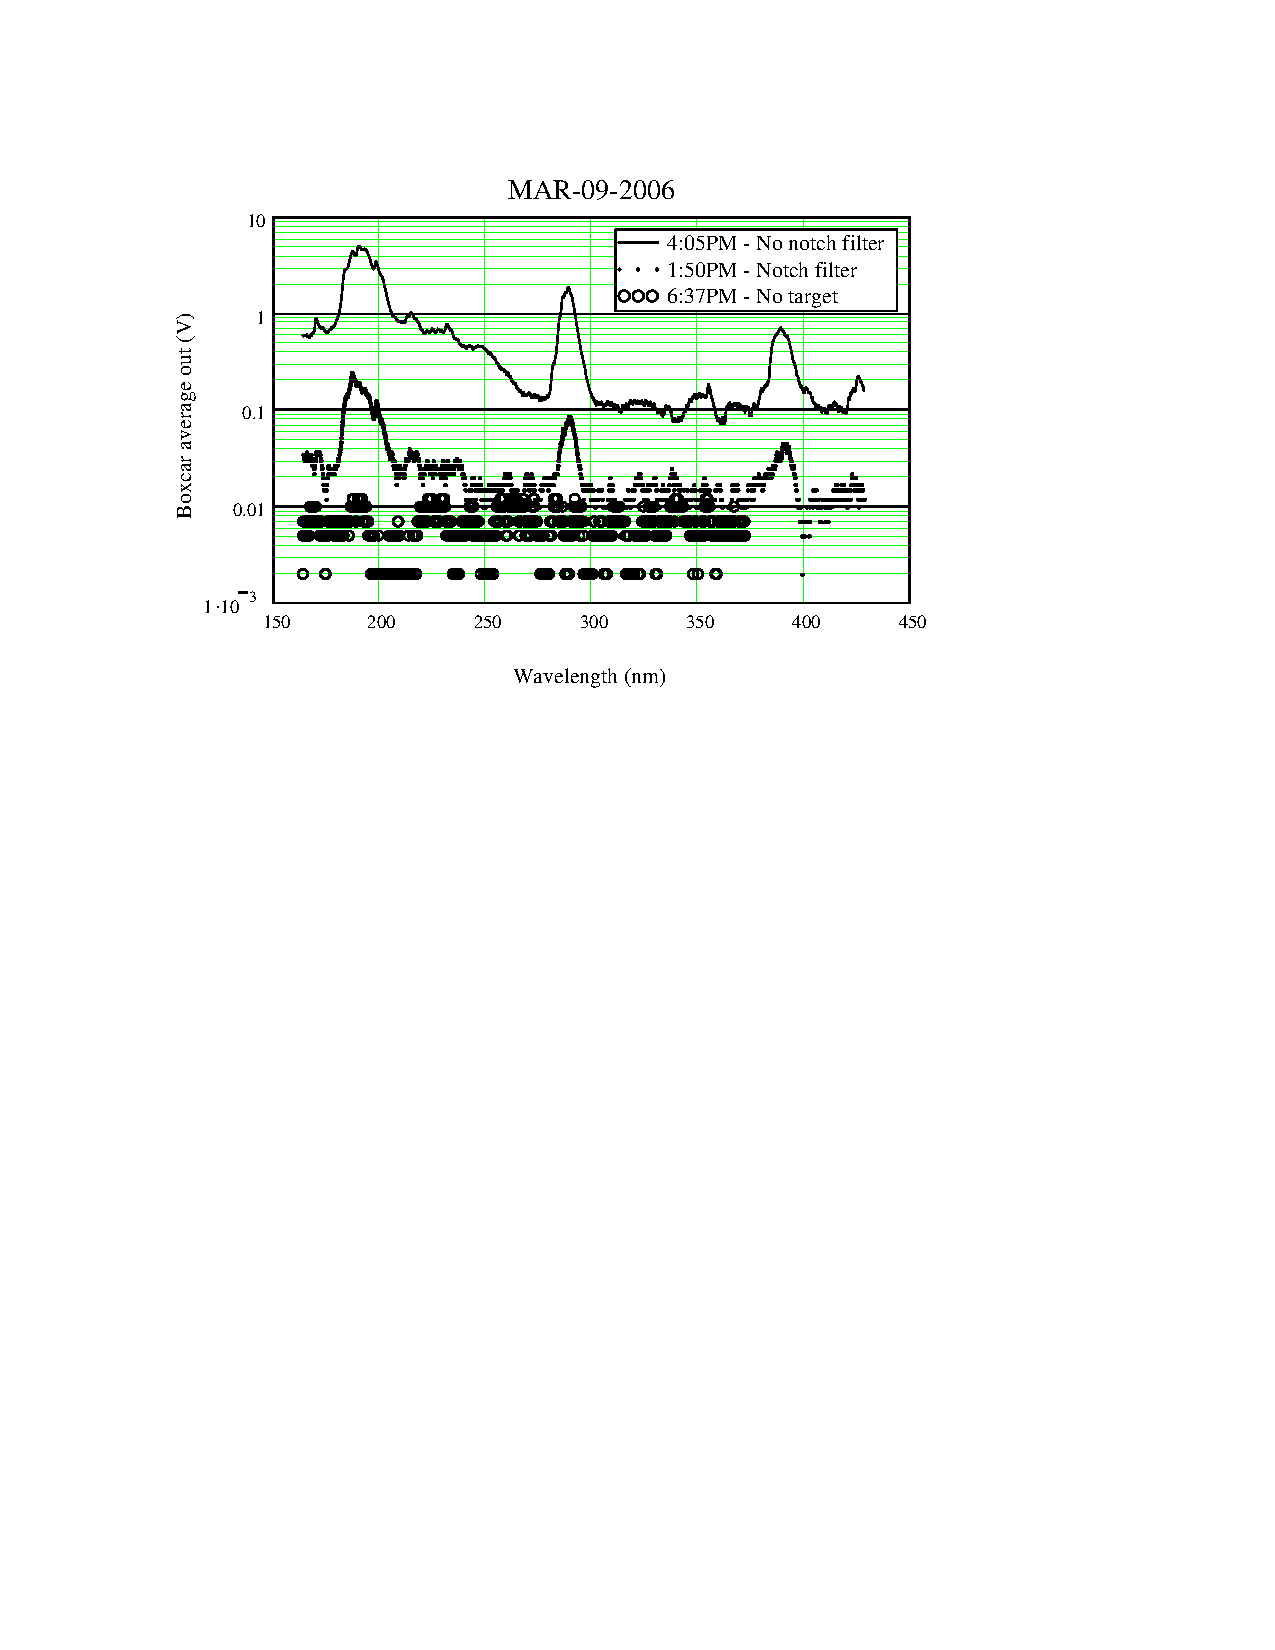
\includegraphics[bb=0 470 489 700]
{1064_ghosts/1064_ghosts.pdf}
}
\caption[Grating ghosts from 1064 nm laser illumination]{Grating ghosts from 1064 nm laser illumination. Using various targets (aromatic compounds, paper, and a calibrated Lambertian target) it was discovered that the spectral ``features'' observed in the UV were independent of the target. Then from the data shown here, acquired using a notch filter made for 1064 nm YAG output, it was concluded that the ``features'' were linearly related in intensity to the 1064 nm excitation and thus most likely ``ghost lines'' associated with the grating.}
\label{1064_ghosts}
\end{figure}
%----------------------------------------------------------------------------
